\documentclass[twoside]{Homework}
\usepackage{graphicx} 

\studname{Si Kai Lee}
\uni{sl3950}
\studmail{sl3950@columbia.edu}
\coursename{Statistical Machine Learning}
\courseno{STAT W4400}
\hwNo{3}

\begin{document}
\maketitle

\section*{Problem 1}
\begin{figure}[!ht]
  \centering
    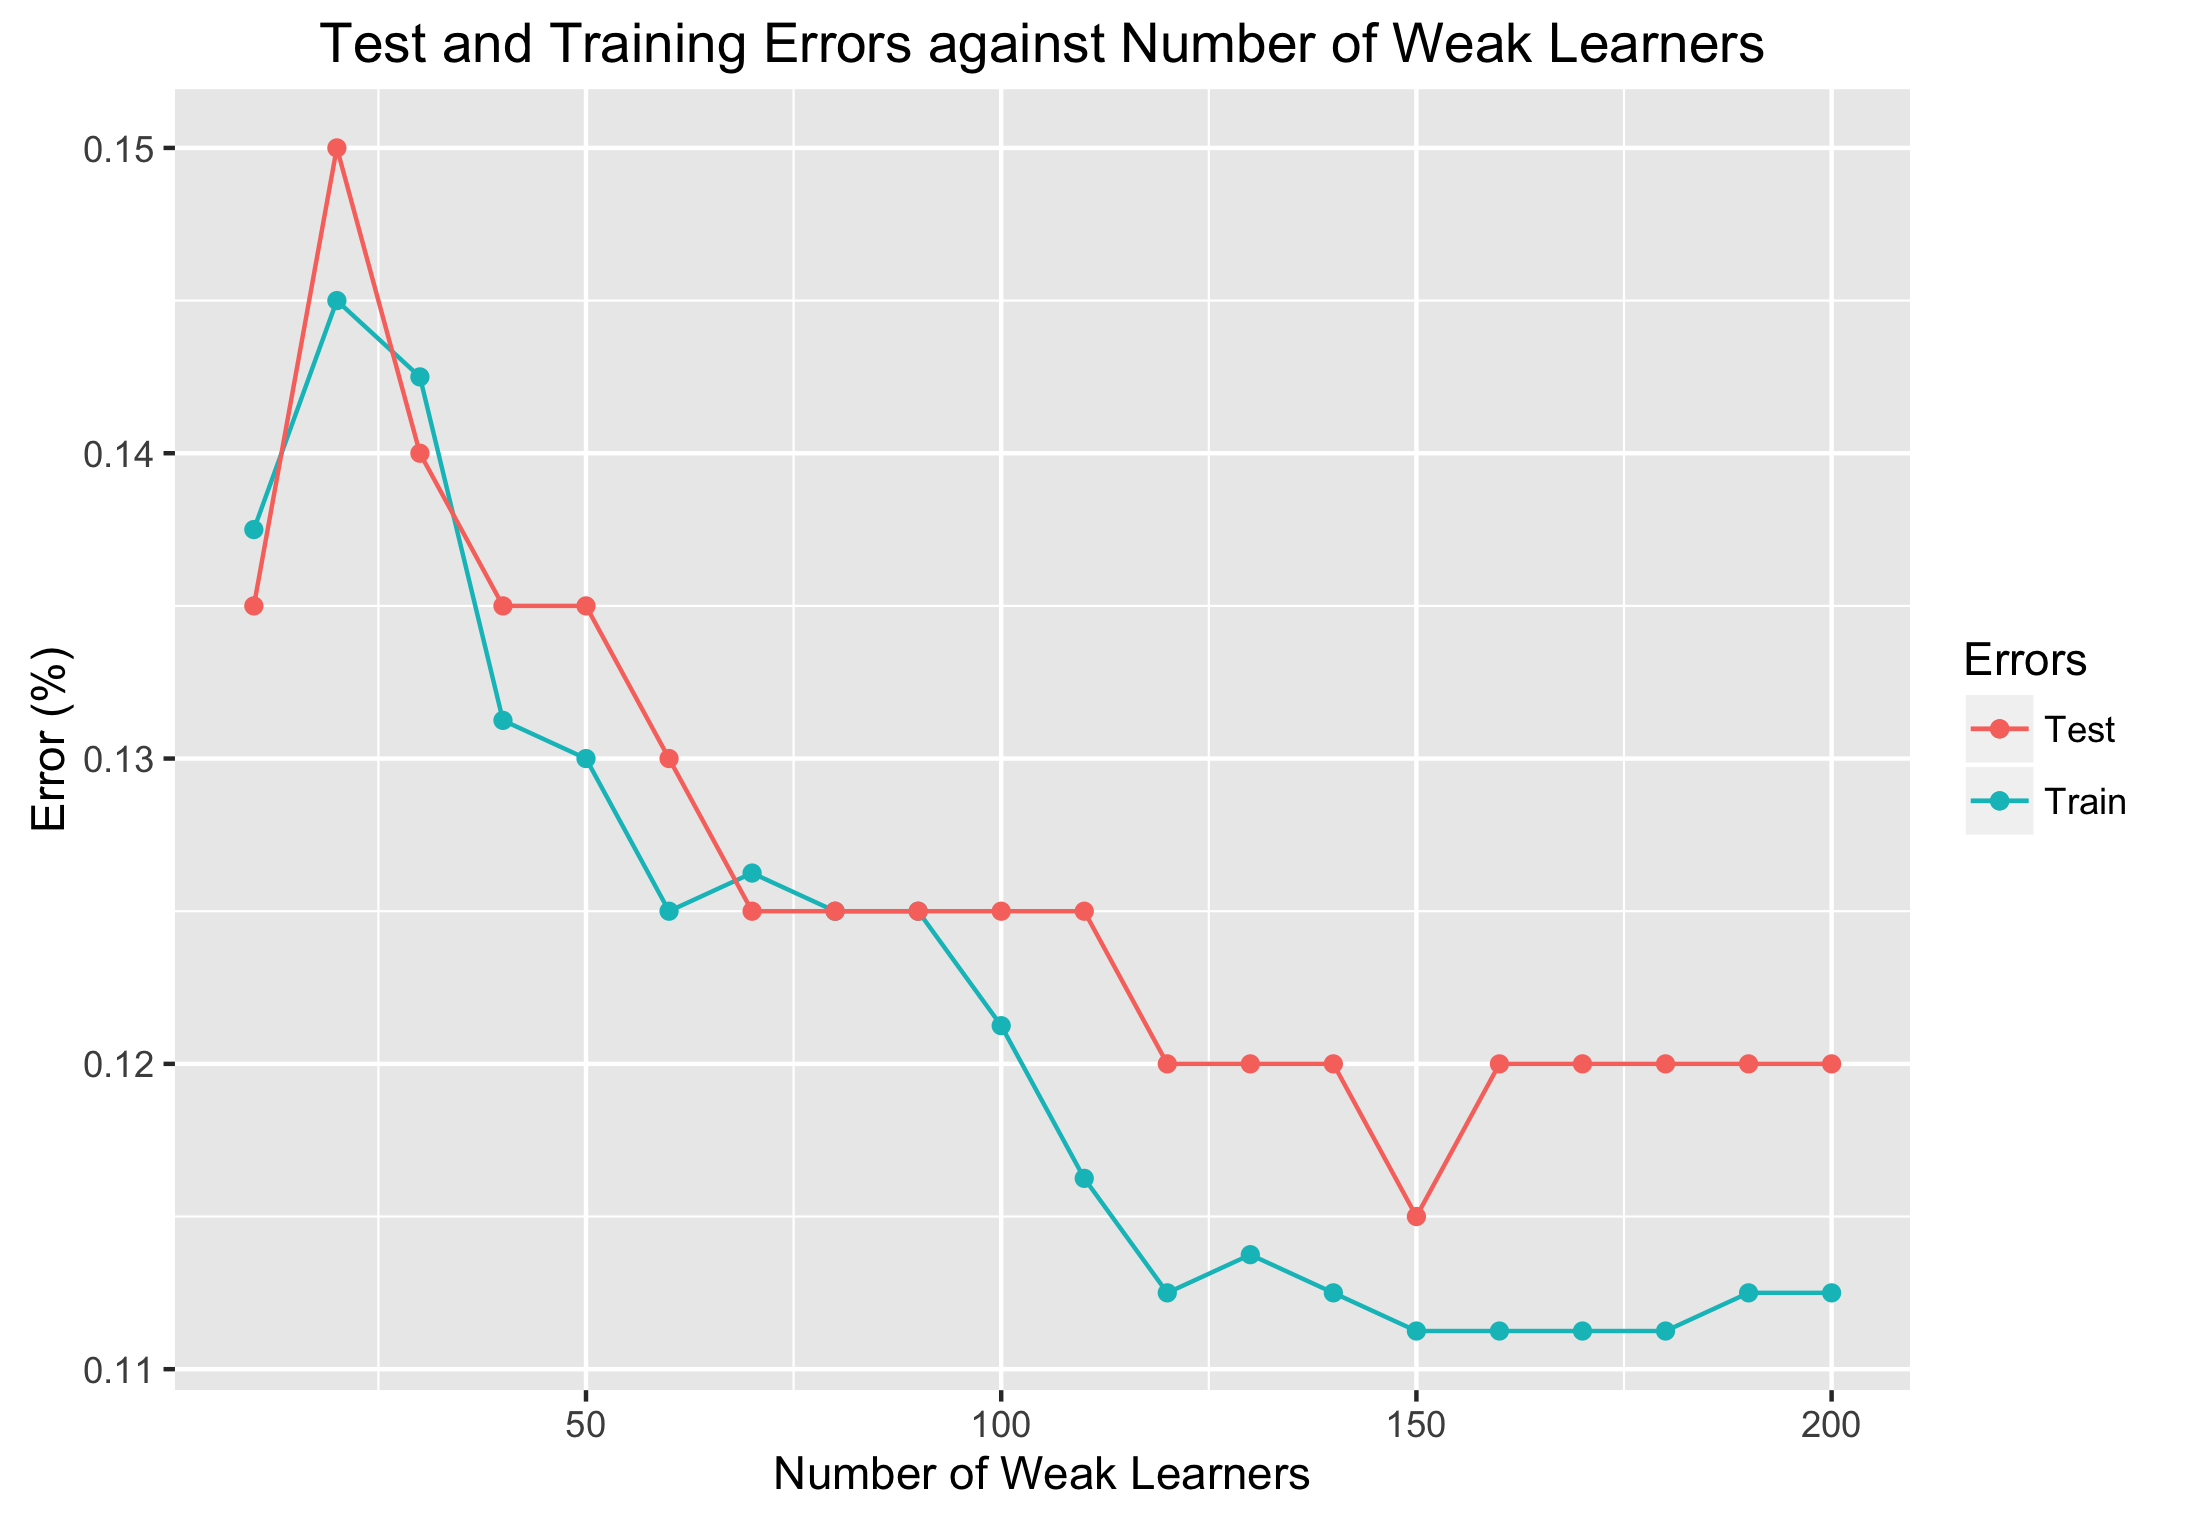
\includegraphics[scale=0.25]{Error_Plot}
  \caption{Training and Cross-Validated Test Errors.}
\end{figure}

\newpage
\section*{Problem 2}
\subsection*{1}
The $\ell_{0.5}$ cost function encourages sparse estimates. Since the tips of the $||\beta||_{0.5}$ constraint region where $\beta_i = 0$ are closest to the contours of least squares error function $||y - X\beta||^2_2$ while the rest of the region curves away from the $||y - X\beta||^2_2$, hence the contours of $||y - X\beta||^2_2$ would most likely intersect with $||\beta||_{0.5}$ at its tips which sets the dimension $\beta_i$ to 0. As the number dimensions increases, the number of tips of the constraint region increases exponentially which increases the likelihood of $||y - X\beta||^2_2$ intersecting at the tips of the constraint region i.e. dimensions being set to 0 and thus results in a sparse estimate.\\
\\\noindent
On the other hand, $\ell_{4}$ cost function does not as the $||\beta||_{4}$ constraint region is a rounded square which curves towards the contours of $||y - X\beta||^2_2$, therefore the two would likely intersect at a point where $\beta_i \neq 0$ so no dimensions would be turned off, leading to non-sparse estimates.

\subsection*{2}
The geometric interpretation of minimising the $\ell_{0.5}$ cost function $\arg \min_{\beta} (||y - X\beta||^2_2 + \lambda ||\beta||_{0.5}^{0.5})$ is equivalent to finding the contours the least squares error function $||y - X\beta||^2_2$ closest to $\beta_{MLE}$ and the smallest $||\beta||_{0.5}$ constraint region. Therefore $x_3$ would achieve the smallest cost as it is the closest point from the contours of $||y - X\beta||^2_2$ which would intersect with $||\beta||_{0.5}$. All other points would only intersect with a larger $||\beta||_{0.5}$ constraint region.\\
\\\noindent
For the second case, $x_4$ would achieve the smallest cost under the $\ell_{4}$ cost function $\arg \min_{\beta} (||y - X\beta||^2_2 + \lambda ||\beta||_{4}^{4})$ as it is the closest point from the contours of $||y - X\beta||^2_2$ which would intersect with a smaller $||\beta||_{4}$ constraint region. All other points would only intersect with the larger $||\beta||_{4}$ shown in the figure on the right.\\

% https://onlinecourses.science.psu.edu/stat857/node/155
\end{document} 